\section{Introduction}
Particle Swarm Optimization (PSO) \cite{pso} is a global optimization technique
inspired by swarm behavior found in nature (e.g., a flock of birds).
Each particle in the swarm moves in a stochastically weighted
combination of two vectors: one in the direction of the best location the
particle has seen locally and one in the direction of the best location seen by
the swarm globally. Here the term ``best'' is with respect to a predefined and
problem specific fitness function.
The swarm maintains a global best position (the position
with the optimal fitness value) and the goal is for this global best position to
converge to the global minimum (maximum).
One of the advantages of PSO is that it searches globally for the optimum,
although it does not have a guarantee of convergence.
In particular, if the particles are initialized in a subspace far from the
global optimum, the change of convergence is greatly reduced.

The challenge comes in the form of required compute power -- due to
the curse of dimensionality, a high-dimensional problem requires a large number
of particles. While improved hardware performance can
improve runtime performance, we have found that efficient algorithm
design coupled with efficient implementation can make similar, if not improved
gains in performance. In the authors'
personal experience, making a heap allocation in the wrong spot or even
something as simple as generating a random number in the wrong location can
have a substantial negative impact on the simulation runtime.\\
The contributions of this work are:

\begin{itemize}
\item An improved cache-efficient algorithm for parallel PSO. In our
  experiments, this improved algorithm obtains $N\times$ speed-ups over the
  naive parallelization of the cache-aware algorithm introduce in
  \cite{cache-pso}.
\item A technique for reducing critical section contention in OpenMP
\item Confirmation of the prior work of Change et al. \cite{cache-pso}

\end{itemize}

While there is a large body of work on parallel PSO using various threading
techniques and GPGPU programming, the goal of our work is to provide a set
of techniques, tools, and modifications to the standard cache-aware PSO
algorithm that are simple to understand and use.
The average PSO implementor
likely does not have the specialized knowledge requried to write an efficient
CUDA implementation or to implement efficient management and coordination of
threads. Rather than provide a highly specialized implementation, we focus on
simplicity and clarity while still improving performance. For parallelism, we
utilize OpenMP. We leave the distributed implementation for future work.

The organization of the paper is as follows. In Section \ref{sec:pso} we give a
breif overview of PSO, followed by a review of prior work in Section
\ref{sec:prior}.
We provide an overview of cache-aware algorithms and introduce the concept of
data oriented design in Section \ref{sec:cache}.
We present our updated PSO algorithm and implementation guidelines in Section
\ref{sec:algo} followed by experimental results in Section \ref{sec:results}.

\section{Particle Swarm Optimization}\label{sec:pso}
Particle Swarm Optimization can be simplified into the update of two formulas:
one for a particle's velocity and the other for the particle's position. Define
$\textbf{pbest}$ as the position corresponding to the best seen fitness value
for a given particle (i.e., the local best), $\textbf{gbest}$ as the position
corresponding to the the best seen fitness value globally, and $\textbf{p}$ as
the current position of the given particle. The update formula for velocity is
given by equation (\ref{eq:velocity} and Table \ref{tab:constants} describes
the interpretation of the constants.

\begin{align}
  \textbf{v}_i(t+1) = \omega \textbf{v}_i (t) & +
                                                c_1 \textbf{r}_1\odot (\textbf{pbest}_i(t) -
                                                \textbf{p}_i(t))
  \\\label{eq:velocity}
  &+ c_2 \textbf{r}_2 \odot(\textbf{gbest}_i(t) - \textbf{p}_i(t))\nonumber
\end{align}

Where $\odot$ is the Haddamard product.
Once the velocity is computed, the position update is given by equation
(\ref{eq:position}).

\begin{equation}\label{eq:position}
  \textbf{p}_i(t+1) = \textbf{p}_i(t) + \textbf{v}_i(t)
\end{equation}

\begin{table}
  \caption{Description of the velocity update constants.}\label{tab:constants}
  \begin{tabular}{ll}\toprule
  \textbf{Constant} & \textbf{Description}\\\midrule
  $\omega$ & Momentum\\
  $c_1$ & Explore towards local best\\
  $c_2$ & Exploration towards global best\\
  $r_1$ and $r_2$ & sampled from $U(0,1)$\\\bottomrule
  \end{tabular}
\end{table}

Algorithm \ref{alg:pso} describes the basic PSO algorithm.

\begin{algorithm}
  \caption{Basic PSO algorithm.}\label{alg:pso}
  \begin{algorithmic}[1]
    \Procedure{PSO}{N}
    \State $\texttt{particles} \gets \texttt{initialize}(N)$
    \Repeat
    \For{$\textbf{p} \in \texttt{particles}$}
    \State $\textbf{gbest} \gets \arg\min_{p\in\texttt{particles}}f(p)$
    \State \texttt{p.UpdateVelocity(\textbf{gbest})}
    \State \texttt{p.UpdatePosition()}
    \EndFor
    \Until Convergence
    \EndProcedure
  \end{algorithmic}
\end{algorithm}

Particles are initialized randomly within the bounds of the search space
$[\texttt{x\_min}, \texttt{x\_max}]$. Particle intialization is an important
step -- if the global optimum is far outside the initialization domain, the
algorithm may not converge to the global optimum.
Some implementations also set a random
intiail velocity for each particle; however, we found it simpler and equally
effective to initialize all particles with zero velocity. In our initial
experiements, we found improved convergence by reflecting particles off the
boundary of a predefined search space using $[x_{\min}, x_{\max}]$. The
reflection was performed by negating the velocity component and offsetting the
particle from the boundary by the amount it would have exceeded the boundary for
the respective position component.
However, we decided to use an open search space with no boundary to give a more
pessimistic view of our algorithm.

Our implementation allows for a predefined minimum and maximum value for
components of the velocity vector -- in practice these should be no greater than
the diameter of the search space.

\section{Prior Work}\label{sec:prior}
There is a large body of work studying the parallelization of PSO. This work can
be broadly broken up into two categories: OpenMP/MPI based methodoligies and
GPGPU based methodoligies (typically via CUDA). OpenMP is a set of pragmas used
with C/C++ or Fortran that automates much of the multi-threading process. MPI
(Message Passing Interface) is a library used for communicating between processes.
The advantage of the OpenMP/MPI
approach is flexibility in parallelization via threads, separate machines, and
frequently both. Additionally, OpenMP/MPI can more easily handle branches
without suffering major performance degradation.
GPGPU approaches are more restricted due to the GPU architecture
-- branching in work groups in a GPU can dramatically reduce performance.\par

The primary challenge in parallelizing PSO is efficiently updating
\texttt{gbest} -- since \texttt{gbest} is a shared resource (and in particular,
shared memory in OpenMP), care must be taken when updating its value. The
simplest solution is to place a lock on \texttt{gbest}; however, the constant
acquisition and subsequent release of the lock will quickly degrade
performance. Dealing with locks is also particularly difficult to get correct,
with subtle, hard to find concurrency bugs being the norm rather than the
exception.

The most common approach to parallelizing PSO is through the use of
sub-swarms. Each sub-swarm is assigned to a thread and sub-swarms share the
sub-swarm best amongst other swarms as a way to communicate
\texttt{gbest}. Many \cite{cooppso, comppso, optionpso}
build the sub-swarm implementation with OpenMP and MPI. Peng et
al. \cite{multicore-pso} also investigate the sub-swarm approach to
parallelization but explore several different swarm communication topoligies and
use Java threading rather than OpenMP and MPI. All works achieve similar linear
speed-ups at low thread counts ($<20$ threads).

The other common approach to parallelizing PSO is via GPGPU programming. The
challenge with GPGPU programming is two-fold: minimizing communication between
the GPU and CPU, which is costly, and avoiding branching within the GPU
kernel\footnote{a kernel in GPGPU programming is the name of the procedure being
  run on  the GPU}. When grouped threads (referred to as a warp) within a GPU
start to diverge due to branching, the
GPU executes one branch at a time.
This can be difficult to avoid in the PSO algorithm where a core part
of the aglorithm is finding the globally optimal particle (i.e., \texttt{gbest}).
To get around this,
some work \cite{gpu-ppso, gpu-pso} uses the GPU primarily for evaluating the
fitness function across all particles simultaneously.
Others, such as Calazan et al. \cite{swarmgrid}, perform the entirety of
the PSO algorithm on the GPU, transferring data from the CPU to the GPU at the
beginning of the algorithm and then transferring the data back to the CPU from
the GPU at the end of the algorithm.
CONTINUE \cite{biopsogpu, multiswarmpso-gpu}

Other recent work \cite{mrcpso, mprso, coop-pso, intrusion-pso} has
studied the use of the MapReduce framework \cite{mapreduce} in parallelizing PSO
for various applications. In most experiments, these works see near linear
scaling with number of nodes added in the MapReduce cluster.
The MapReduce implementations serve as a complementary
approach to the CPU and GPU-based work. For example, each node in the MapReduce
cluster can run an OpenMP and/or
GPGPU-based algorithm. Improvements to the CPU and GPU PSO algorithms directly
flow into the work of the MapReduce-based algorithms. A similar approach of using
MapReduce for coarse-grain parallelism and resiliency while allowing
models to manage the fine-grained
parallelism is also being investigated by the deep learning community \cite{mrpnn,
  heterospark, dlspark}. 

\section{Cache-aware Design}\label{sec:cache}
Modern x86\_64 CPUs typically have three tiers of cache: L1, L2, and
L3. L1 cache is the fastest but has the smallest amount of storage. The caches
decrease in speed and increase in storage as one descends the cache
hierarchy (with L3 being the lowest). When data is to be loaded into a register,
the CPU first checks the
cache, then RAM, and lastly disk. Rather than load a single piece of data from
RAM into cache, CPUs load a cache line, which is typically 64B, which
corresponds to 16 32-bit numbers or 8 64-bit numbers. A cache-aware
algorithm utilizes this information by grouping data such that data utilized by
the algorithm in temporal proximity is stored physically close together. This
is referred to as data locality. In other words, we want to keep data that is
accessed at around the same time as close together as possible. Doing so reduces
access to RAM and disk, both of which are substantially more
costly than accessing cache.

\subsection{Data-Oriented Design}
We can use the idea of data locality to
influence the design of our programs. This is one aspect of what is known as
data-oriented design and
is a very common technique in the video game industry, which is known for
writing performant code.
Data-oriented design
differs from object-oriented design in that data is grouped based on access
paterns rather than logical patterns.

\begin{figure}
  \lstinputlisting{../code/particle.cpp}
  \caption{Example of a Particle class using object-oriented
    design.}\label{fig:particle}
\end{figure}

Figure \ref{fig:particle} shows a typical object-oriented implementation of PSO.
The information specific to a particle is logically grouped together. From a
design point of view, this is a sensible approach. However, as we will see
later, from a performance point of view this is a costly design choice with
respect to performance.
When a particle gets loaded into cache from memory, the
cache line will contain three \texttt{T*}\footnote{\texttt{T} is either a float
  (32 bits) or a double (64 bits)} pointers, the three constant values
$c_1$, $c_2$, and $\omega$, and three function pointers to the fitness,
position, and velocity update functions.

Figure \ref{fig:particles} shows an example of one possible data-oriented design
approach. The key aspects with this design are that particle positions are stored
in a vector, particle velocities are stored in a vector, and particle best
positions are stored in a vector. Rather than encapsulate particle specific
information in a particle object, we place that information in a vector along
with similar information of other particles. The advantage is data
locality with the tradeoff of increased book-keeping.
The data locality means when the velocity or position for a given particle is
loaded into cache, we also get the data for its neighbors loaded into cache for
free. 
For example, when the first velocity vector (we
can think of this is a \texttt{T*} pointer), the next seven
velocity pointers will also be pulled into cache because they are on the same
cache line. Compare this with the object-oriented approach where we would need
seven different loads from main memory to get these pointers since each particle
object takes up an entire cache line.
\subsection{Terminology}
The OOP design is sometimes referred to as \emph{array of structs} (AoS) while
the data-oriented design is referred to as \emph{struct of arrays} (SoA).
We use this terminology and add a third: SoA - efficient, which
represents the efficient, data-oriented design. These names are summarized in
Table \ref{tab:names}

\begin{table}
  \centering
  \caption{Description of algorithm names.}
  \label{tab:names}
  \begin{tabular}{ll}\toprule
    \textbf{Name} & \textbf{Description}\\\midrule
    AoS & Array of Structs - Object Oriented\\
    SoA & Struct of Arrays - Data Oriented\\
    SoA - efficient & Efficient Struct of Arrays\\\bottomrule
  \end{tabular}
\end{table}

          

\begin{figure}
  \lstinputlisting{../code/particles.cpp}
  \caption{Example of a data-oriented design modeling all particles in a PSO
    simulation.}\label{fig:particles}
\end{figure}

\begin{algorithm}
  \caption{Cache-aware algorithm for PSO.}\label{alg:pso-cache}
  \begin{algorithmic}[1]
    \Procedure{PSO-DO}{N}
    \State $\texttt{vel} \gets \texttt{initialize}(N)$ \Comment{velocity vectors}
    \State $\texttt{pos} \gets \texttt{initialize}(N)$ \Comment{position vectors}
    \State $\texttt{bpos} \gets \texttt{pos}$ \Comment{best position vectors}

    \Repeat
    \State $\texttt{gbest} = \text{argmin}_{\texttt{pos}}\texttt{fitness}(p)$
    \For{$i = 0 \to \texttt{n\_particles}$}
    \State $p \gets \texttt{pos}[i]$
    \State $v \gets \texttt{vel}[i]$
    \State $\texttt{local} \gets (\texttt{pos}[i] -
    \texttt{bpos}[i])$
    \State $\texttt{global} \gets  (\texttt{pos}[i]
    - \texttt{gbest})$
    \State $v \gets \omega v + c_1 r_1 \texttt{local}  + c_2 r_2 \texttt{global}$
    \State $p += v$
    \If{$\texttt{fitness}(p) < \texttt{bpos}[i]$}
      \State $\texttt{bpos}[i] \gets p$
      \If{$\texttt{fitness}(p) < \texttt{fitness}(\texttt{gbest}$}
      \State $\texttt{gbest} \gets p$
      \EndIf
    \EndIf
    \EndFor
    \Until convergence
    \EndProcedure
  \end{algorithmic}
\end{algorithm}

\section{Cache-aware Parallel PSO}\label{sec:algo}
We make several improvements to the framework for cache-efficient PSO proposed
in \cite{cache-pso}. While none of these improvements is a major structural
change to the algorithm of PSO or the data-oriented design, we found that the
net effect was a dramatic improvement in performance.

\paragraph{Random Weights} One of the major speed-ups we achieved was through
the generation of the random weights $r_1$ and $r_2$. The original description of
PSO \cite{pso} has two calls to \texttt{rand()} during the velocity update for each
component of the velocity vector. We surveyed a number of highly cited works in
PSO literature \cite{pso-development, pso-overview, pso-tutorial} and found in
all descriptions of the algorithm the random values $r_1$ and $r_2$ are sampled
for each element of $\textbf{v}$ (i.e., for $\textbf{v}\in\mathbf{R}^n$ there
are $n$ unique values of $r_1$ and $n$ unique values for $r_2$). We modify this
approach to use a single value $r_1$ and a single value for $r_2$ for all
components of \textbf{v}. Additionally, in the effecient implementation, we batch
the generation of these values once per system update, rather than generating
them for each vector.
There are two advantages to this approach: we can keep
these random values in cache and we avoid expensive calls to random number
generation routines. This can be seen in Figures \ref{fig:naive-par} and
\ref{fig:efficient-par}. The naive approach, shown in Figure \ref{fig:naive-par}
makes two calls to
\texttt{random\_uniform} for each particle. The efficient, shown in Figure
\ref{fig:efficient-par},
approach indexes the $r$-value vectors \texttt{r1s} and \texttt{r2s}, which are
created at the start of each call to \texttt{UpdateVelocity}. Some readers may
note that this is a rather obvious optimization -- we agree. However, in
practice it seems it is an optimization that is frequently overlooked.
Another potential criticism of this approach is that it reduces variation in the
updated velocity, which could potentially slow convergence. In our experience,
the speed-up gained by using a single $r_1$ and $r_2$ outweighs any slowed
convergence resulting from reduced diversity.\par
We could further improve performance be passing in a pre-allocated vector to the
random number generating routine. However, this makes the code a little more
opaque since it is not always clear a return parameter is returning a
value. Additionally, it is possible that in some cases the compiler is eliding
this allocation on its own.

\paragraph{Reducing Critical Section Contention} Updating \texttt{gbest}
requires checking all particles against the current \texttt{gbest} and updating
when a position with a better fitness value is found. This is a classic
reduction scenario, which can be done in $O(\lg n)$ time. OpenMP provides the
facilities to handle this efficiently, but only for a few simple types and
operations. Unforutnately, these do include \texttt{std::vector<T>}. To get
around this we do a linear scan of all particles in parallel. This presents its
own challenge due to the data race that occurs when multiple threads attempt to
update \texttt{gbest}. Figure \ref{fig:naive-update} shows an example of a
standard use of OpenMP's \texttt{critical} section to avoid the data race. This
reduces performance because the critical section is hit for every particle on
every update. Inspired by the work on distributed deep learning [CITE], where
they perform asynchronous updates in a manner such that distributed workers are
not guaranteed to have the latest information, we use two nested if-statements
with the \texttt{criticle} section on the inner statement, as shown in Figure
\ref{fig:efficient-update}. The intuition behind this is quite simple -- rather
than take a hit on the \texttt{critical} section for every single particle, we
have all particles first check if they could possibly be the best global
partical by checking against the current \texttt{gbest}. If this fails, they
miss the critical section and move on. In the even the first check passes, the
particle then hits the \texttt{critical} section. As demonstrated in our
experiements, this produced a substantial speed-up.

Although we are able to avoid ctirical section contention for a number of the
particles, we introduce a separate issue. The updates to \texttt{gbest} are not
atomic. It is possible for one thread to be reading the value of
\texttt{gbest} while another thread is updating it. This has two primary
consequences. First, some particles may use an incorrect \texttt{gbest} when
computing the velocity update. Second, some particles that are currently the true
\texttt{gbest} may skipp the critical section if they read an incorrect value of
\texttt{gbest} that results in a lower fitness value. Both of these issues
result in a slower rate of convergence. Despite the slower rate of convergence,
the actual wall-clock time is substantially faster. Similar to the asynchronous,
distributed deep learning algorithms [CITE], we trade reduced convergence for
faster runtime.


\begin{figure}
  \lstinputlisting{../code/efficient_update.cpp}
  \caption{Efficient update in a critical section for the efficient parallel PSO
    algorithm.}
  \label{fig:efficient-update}
\end{figure}

\begin{figure}
  \lstinputlisting{../code/naive_update.cpp}
  \caption{Naive update in a critical section for the naive parallel PSO
    algorithm.}
  \label{fig:naive-update}
\end{figure}

\begin{algorithm}
  \caption{Cache-aware parallel PSO}\label{alg:par-pso}
  \begin{algorithmic}[1]
    \Procedure{Parallel-PSO}{N}
    \State $\texttt{n\_threads} \gets \texttt{getn\_hardware\_threads}()$
    \State $\texttt{tp} \gets \texttt{ThreadPool}()$
    \State $\texttt{vel} \gets \texttt{initialize}(N)$
    \State $\texttt{pos} \gets \texttt{initialize}(N)$
    \State $\texttt{bpos} \gets \texttt{pos}$

    \State $n = N/\texttt{n\_threads}$ \Comment{Assume $N \mod
      \texttt{n\_threads} = 0$}
    \For{$(i, t) \in \texttt{enumerate}(\texttt{tp})$}
    \State $vs \gets \texttt{vel}[ni:n(i+1)]$
    \State $ps \gets \texttt{pos}[ni:n(i+1)]$
    \State $bps \gets \texttt{bpos}[ni:n(i+1)]$
    \State $\texttt{t(Run}(vs, ps, bps))$
    \EndFor
    \For{$t \in \texttt{tp}$}
    \State \texttt{t.join()}
    \EndFor
    \EndProcedure
  \end{algorithmic}
  \begin{algorithmic}[1]
    \Procedure{Run}{\texttt{vs}, \texttt{ps}, \texttt{bps}}
    \State $n \gets \texttt{ps.size()}$
    \Repeat
    \For{$i = 1 \to n$}
    \State $\texttt{gbest} \gets \min\{\texttt{gbest}, \texttt{po}$
    \EndFor
    \For{$i = 1 \to n$}
    \State 
    \EndFor
    \Until convergence
    \EndProcedure
  \end{algorithmic}
\end{algorithm}

\begin{figure}
  \lstinputlisting{../code/naive_par.cpp}
  \caption{Naive loop parallelization with OpenMP.}\label{fig:naive-par}
\end{figure}

\begin{figure}
  \lstinputlisting{../code/efficient_par.cpp}
  \caption{Efficient loop parallelization with OpenMP.}\label{fig:efficient-par}
\end{figure}

\section{Results}\label{sec:results}
\begin{table}
  \centering
  \caption{Test functions used in experiments.}\label{tab:functions}
  \begin{tabular}{ll}\toprule
    \textbf{Name} & \textbf{Function}\\\midrule
    Ackley & $-20\exp\Big(-0.2\sqrt{\frac{1}{n}\sum_ix_i^2}\Big)$ -\\
    & \hspace{5mm} $\exp\Big(\frac{1}{n}\sum_i\cos(2\pi x_i)\Big) + e + 20$\\
    Quadratric & $\sum_i x_i^2$\\
    Rastrigin & $10n + \sum_{i=1}^n(x_i^2 - 10\cos(2\pi x - i))$\\\bottomrule
  \end{tabular}
\end{table}
We test our algorithm on several popular test functions in optimization
\cite{testprobs} the the quadratic, Rastrigin
\cite{rastrigin}, and Ackley \cite{ackley} functions, shown in Table
\ref{tab:functions} generalized to $\mathbb{R}^n$. All of these functions have
the property that their minimum is attained at the origin with a value of
$0$, which makes assessing the models easy. Three-dimensional plots of the
Rastrigin and Ackley functions are shown in figures \ref{fig:rastrigin} and
\ref{fig:ackley}, respectively.
All experiments were run on a single
workstation with a 6-core, 3.6 GHz Intel i7-6800K processor with 64GB of RAM. We
used six threads in OpenMP, rather than 12 hyperthreads, to reduce context switching.
Table \ref{tab:param}
gives the hyperparameters used in the experiements. These were chosen based on
the recommended values from \cite{pso-convergence, spso} -- the advantage of
using these parameters is that they do not need tuning. It is
worth noting that in our experience these parameters work well but performance
can frequently be improved via tuning.

\begin{table}
  \centering
  \caption{Hyperparamters used in the experiements.}\label{tab:param}
  \begin{tabular}{lc}\toprule
    \textbf{Parameter} & \textbf{Value}\\\midrule
    $c_1$ & $2.05 \chi$\\
    $c_2$ & $2.05 \chi$\\
    $\omega$ & $\chi$\\
    $\chi$ & $\frac{2}{2.1 + \sqrt{.41}}$\\\bottomrule
    \end{tabular}
\end{table}

Bratton et al. \cite{spso} mention that particles should be initialized away
from the target global optimum to prevent unintentional bias as a result of
particles being initialized close to the optimum. However, since our
distributions have their optimums at the origin, moving to a higher dimensional
space means that particles randomly intialized from a uniform distribution will
cluster towards the outer edges of the search space (see, for example, ``curse
of dimensionality'' \cite{hastie}). Empirically, in $\mathbb{R}^{10}$, the
probability a point being randomly initialized within $\text{diam}/2$ of the origin is 0.1 \%.
We verified this experimentally and found no
impact to runtime when sampling initial positions from $U(x_{\min}, x_{\max})$
and from $U((x_{\min},\lambda x_{\min})\cup(\lambda x_{\max}, x_{\max}))$.

\begin{table}
  \centering
  \caption{Sequential speed-up with respect to Array of Structs design (dimension
    75 with 500 particles.)}
  \label{tab:seq-baseline}
\begin{tabular}{llll}\toprule
Structure       & Ackley & Rastrigin & Quadratic \\\midrule
SoA             & 25.5\%  & 29.2\%     & 10.4\%     \\
SoA - efficient & 44.7\%  & 46.2\%     & 57.0\%     \\\bottomrule
\end{tabular}
\end{table}

Table \ref{tab:seq-baseline} shows the sequential speed-up with respect to the
AoS design for 500 particles in $\mathbb{R}^{75}$. The SoA architecture as
proposed in \cite{pso-cache} results in strong improvements of the AoS
architecture. More interesting is the improvement of the SoA - efficient
architecture. Because these results are for sequential algorithms, the speed-up
of the SoA - efficient algorithm is primarily due to batching the random number
generation.


\begin{figure}
  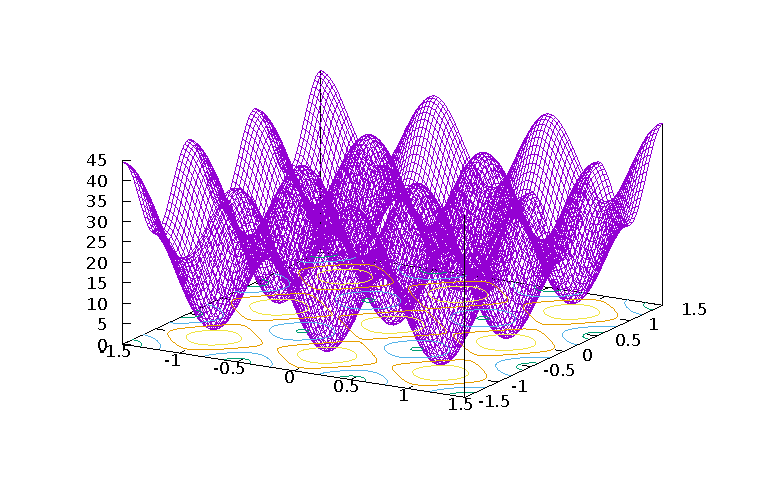
\includegraphics[width=\columnwidth]{../img/output/rastrigin}
  \caption{The Rastrigin function in three dimensions.}\label{fig:rastrigin}
\end{figure}

\begin{figure}
  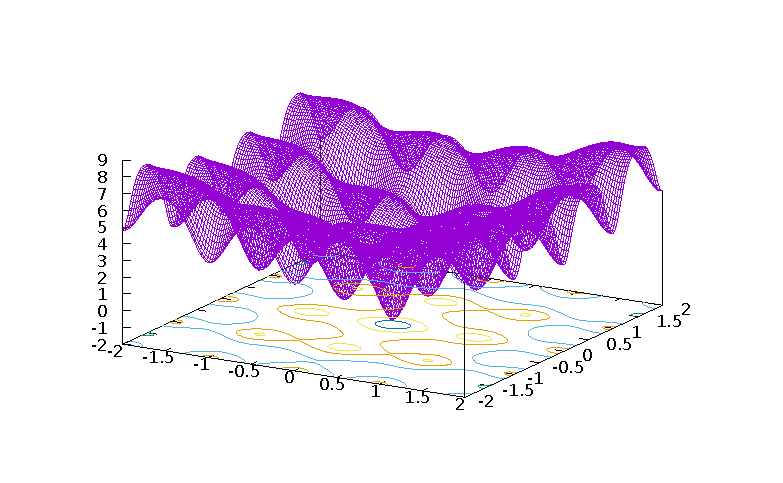
\includegraphics[width=\columnwidth]{../img/output/ackley}
  \caption{The Ackley function in three dimensions.}\label{fig:ackley}
\end{figure}

Figures \ref{fig:exp-dim} and \ref{fig:exp-N} compare the performance impact of
increasing the dimensions and the number of particles in the system,
respectively. [NOTE: re-run or check the numbers of
\ref{fig:exp-dim}]. Interestingly, SoA - efficient, seems to handle increasing
particle dimensions better than SoA and AoS. On closer inspection, this behavior
is quite intuitive. Observe that in Figure \ref{fig:efficient-par}, we allocate
an entire vector for the random weights, one weight for each particle. This
allocation occurs for each update of the system, which could be arbitrarily
large. This is an example of where it may be worth passing in pre-allocated
vectors (i.e., \texttt{r1s} and \texttt{r2s}), rather than generating new
vectors each iteration.


\begin{figure}
  \includegraphics[width=\columnwidth]{../img/output/dim}
  \caption{Results of the increasing dimension experiments with 1,000
    particles.}
  \label{fig:exp-dim}
\end{figure}

\begin{figure}
  \includegraphics[width=\columnwidth]{../img/output/N}
  \caption{Results of increasing the number of particles for a fixed dimension
    size of 100.}
  \label{fig:exp-N}
\end{figure}

\begin{table}[]
  \caption{Parallel results for dimension 100 with 1,000 particles limited to
    $10^6$ steps. Note: speed-up is with respect to the sequential version of
    the algorithm.}
  \label{tab:results}
\begin{tabular}{lllll}\toprule
  &                           & \textbf{AoS}             & \textbf{SoA}         & \textbf{SoA - efficient}     \\\midrule
\multicolumn{2}{l}{\textbf{Ackley}}    &                         &                         &                     \\
  & Time (s)                  & $310 \pm 7$             & $236 \pm 27$            & $149 \pm 30$        \\
  & Fitness                   & $1.7 \pm .7$           & $1.5 \pm .8$            & $1.9 \pm .4$        \\
  & Speed-up  & 2.7                     & 2.31                    & 2.95                \\
\multicolumn{2}{l}{\textbf{Quadratic}} &                         &                         &                     \\
  & Time (s)                  & $359 \pm 6$             & $286 \pm 7$             & $56 \pm 2$          \\
  & Fitness                   & $4.0 \pm .5 \cdot 10^{-6}$ & $7.0 \pm .5 \cdot10^{-7}$
                                                                 &
                                                                            $2.0
                                                                   \pm .2 \cdot
                                                                            10^{-5}$ \\
  & Speed-up  & 1.5                     & 1.75                    & 5.96                \\
\multicolumn{2}{l}{\textbf{Rastrigin}} &                         &                         &                     \\
  & Time (s)                  & $296.8 \pm .6$          & $209.5 \pm .3$          & $122 \pm 3$         \\
  & Fitness                   & $192 \pm 47$            & $170 \pm 24$            & $170 \pm 46$        \\
  & Speed-up  & 5.75                    & 6.25                    & 8.38           \\\bottomrule    
\end{tabular}
\end{table}

Table \ref{tab:results} shows the results of the three parallel versions of the
algorithms for a fixed system size of 1,000 particles in $\mathbb{R}^{100}$
averaged over 20 runs. The simulations were limited to $10^6$ steps due to
compute resource limitations. 
Unfortunately, for Rastrigin and arguably Ackley, $10^6$ stpes was not sufficient.
It should be noted that the sequential Rastrigin
simulation failed to converge to the global minimum of $\mathbf{0}$ as well.

The SoA - efficient algorithm demonstrated the best scalability, achieving more
than an $8\times$ speed-up for Rastrigin. Recall that the experiments were run
using six physical cores, yet we see a speed-up greater than $6\times$. This is
due to additional compiler optimizations. As stated previously, we used
link-time optimizations and loop unrolling, in addition to compiler-generated
AVX instructions. The longer the simulation runs, the greater the impact of
these optimizations. Additionally, as stated previously, the simulations run for
a maximum of $10^6$ steps or convergence, whichever comes first. Neither Ackley
nor Rastrigin converged to a suitable solution, which means they both hit the
maximum step limit. However, they have very different run-times, with Ackley
being anywhere from 2\% to 20\% slower. The difference in speed is due to
fitness function evaluation -- more time is spent evaluating the fitness
function in Ackley while, which means the increased performance from multiple
threads and AVX instructions has less of an impact on the overall
performance. Conversely, since Rastrigin has a relatively simpler fitness
function, it experiences a greater performance boost as a result of spending
more time looping over the particles (via multiple threads) and updating the
components of the particles (threads and AVX instructions).

\section{Conclusion}
In this work we present two optimizations to improve the performance of both the
standard and parallel version of the PSO algorithm. At a minimum, this work
introduces specific guidance on how and where to generate the random weights in
PSO, which, as we demonstrated, results in substantial performance gains. The
technique introduced to avoid ctricial section contention is also widely
applicable to other algorithms.

Two avenues for future work are investingating the asynchronous, multiple
machine implementation and expanding this work to other algorithms such as Ant
Colony Optimization and genetic algorithms. Specifically, it would be
interesting to expand the critical section contention technique to a
message-passing paradigm where communication and coordination patterns can
become quite complex.


